Radioactivity is the process in which an unstable atomic nucleus loses energy through the emission of particles such as photons, electrons, etc. This process has been present in the Universe since its inception as it was an important process of the Big Bang\footnote{The Big Bang is the most acceptable hypothesis that explains the formation of the universe and its development over time so far.}. This was also present during the formation of the earth which explains why the different layers that make up the earth contain radioactive elements. 

Humanity has always been exposed to radioactivity, whether present in the Earth's crust or in extraterrestrial sources (external natural irradiation). The human being himself is radioactive as radioactive elements are contained in the human body such as $\ce{^{3}H}$, $\ce{^{14}C}$ or $\ce{^{40}K}$, introduced into the body through food or water ingestion or air inhalation (internal natural irradiation). The annual average radioactive dose received by the world population is presented in Figure \ref{fig:RadioactiveDosePopulation} and Table \ref{tab:RadioactiveNaturalDosePopulation}.

\begin{figure}[h]
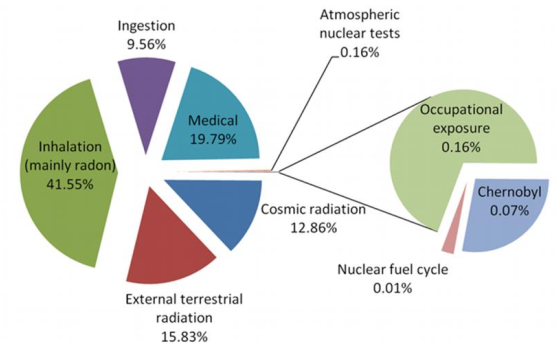
\includegraphics[scale=0.5]{2Introduction/RadioactiveDosePopulation.png}
\centering
\caption{Annual average distribution of the radioactive dose received by the population~\cite{IAEA}\label{fig:RadioactiveDosePopulation}.}
\end{figure}

\begin{table}[htbp]
\centering{}%
\begin{tabular}{lcc}
\toprule 
Radiation source & Eff. dose ($\milli\sievert/$yr) & Typical range ($\milli\sievert/$yr)\tabularnewline
\midrule
\midrule 
Cosmic (external) & $0.39$ & $0.3 - 1.0$ \tabularnewline
terrestrial (external) & $0.48$ & $0.3-0.6$ \tabularnewline  
Inhalation (internal) & $1.26$ & $0.2-10$ \tabularnewline
Ingestion(internal) & $0.29$ & $0.2-0.8$ \tabularnewline
\midrule
Total & $2.42$ & $1-12.4$ \tabularnewline
\bottomrule
\end{tabular}
\caption{Annual average distribution of the effective dose received by the population due to natural radioactivity~\cite{UNSCEAR, CSN}.}
\label{tab:RadioactiveNaturalDosePopulation}
\end{table}

As it can be seen in Figure \ref{fig:RadioactiveDosePopulation}, most of the radioactive dose received by the population is due to both internal and external natural radiatioactivity, the effective dose\footnote{The effective dose is the radioactive dose absorbed by the population, taking into account the different radiosensitivity of each organ or tissue.} of which is estimated to be $2.42~\milli\sievert/$yr as shown in Table \ref{tab:RadioactiveNaturalDosePopulation}. 

Since the discovery of radioactivity by Heri Becquerel in $1896$, lots of nuclear-based technology has been developed and applied to several fields such as energy production, research, medicine, industry, etc. Due to this nuclear technological development, various anthropogenic radioactive sources have appeared in society, resulting in a greater amount of radioactive elements released to the environment. It can be noticed in Figure \ref{fig:RadioactiveDosePopulation} that the most important part of the dose received by the population from artificial sources comes from medical practices. The growing knowledge and development of measurement techniques of radioactivity, enable better assessment and characterization of the harmful effects of radioactivity in living organisms. Because of that, it is important to control the level of radioactive background to which the population is exposed and to ensure that these levels are kept below a safe limit. To accomplish this task, several organizations were created to propose recommendations in radiological protection to the different state organisms and governments at the international level:

\begin{enumerate}
\item{} A definition of concepts and units was necessary to quantify the negative effects of radioactivity and, for that, the International Commission of Radiological Units and Measurements, ICRU \cite{ICRU}, was created during the first international conference of radiology held in London, in 1925.

\item{} The International Commission on Radiological Protection, ICRP \cite{ICRP}, was created in 1928 by the International Society of Radiology, ISR \cite{ISR}. The ICRP aims to make recommendations and to provide guidance on different aspects of protection against radioactivity. The ICRP does not have the legal capacity to enforce its recommendations, but these are widely included in the legislation of most countries. %is fairly consistent with them.

\item{} The United Nations Scientific Committee on the Effects of Atomic Radiation, UNSCEAR \cite{UNSCEAR}, was created in 1955, with the goal of estimating and reporting the levels and effects of ionizing radiation on the population and the environment. These estimates are taken into account by governments worldwide to establish their safety standards.

\item{} The International Atomic Energy Agency, IAEA \cite{IAEA}, was created in 1957 to promote the peaceful use of nuclear energy and to avoid its use for military purpose such as nuclear weapons. Although IAEA is an independent agency, it must to periodically report to the United Nations, (UN) \cite{UN}.

\item{} At the level of the European Union (EU), the European Atomic Energy Community (EURATOM) was created in 1957, which is an international organization created through and ruled by the EURATOM treaty. Its objective is to coordinate research programs for the peaceful use of nuclear energy and the sharing of knowledge, infrastructure and funding of nuclear energy.

\item{} In Spain, the Nuclear Safety Council (CSN) was created in 1980 \cite{CSN}. The CSN is the only authority in Spain on nuclear safety and radiation protection and its objective is to protect employees, the general population and the environment from the harmful effects of ionising radiation from anthropogenic origins. For this task, the CSN ensure that nuclear and radioactive facilities are operated safely and establish the preventive and corrective measures to apply in all radiological emergencies. The CSN has created various networks consisting of several detectors of radioactivity that are in charge of controlling the levels of radioactivity in the environment and assessing the impact of radioactivity facilities. Two of the most important networks are the network of automatic stations (REA, "Red de Estaciones Automáticas") and the network of sampling stations (REM, "Red de Estaciones de Monitoreo"):

\begin{enumerate}
\item{} The network of automatic stations, REA \cite{REA}, shown in Figure \ref{subfig:REA}, consists of several gamma detectors\footnote{Detectors that only measure gamma radioactivity} distributed in Spain that measure the radioactive dose in real time. The REA is employed for real-time detection of radiological issues, which enable taking prompt safety measures.

\item{} The network of sampling stations, REM \cite{REM}, shown in Figure \ref{subfig:REM}, consists of several strategic points in Spain where samples are taken and transported to a laboratory to be measured. About twenty Spanish laboratories integrate this network, the objective of which is to characterize the concentration and evolution of various radioisotopes present in the radioactive background of Spain and to quantify the impact of radioactive facilities on the environment.
\end{enumerate}

\begin{figure}
\centering
    \begin{subfigure}[b]{0.7\textwidth}
    \centering
    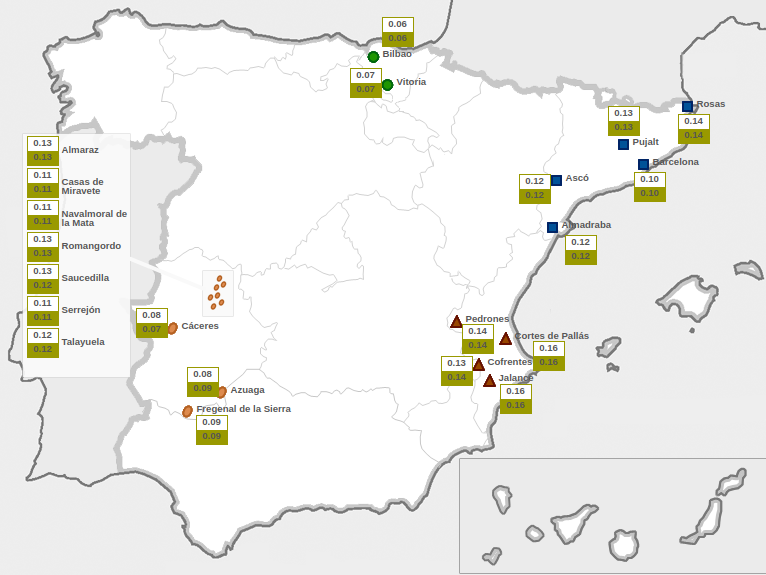
\includegraphics[width=\textwidth]{2Introduction/REA.png}  
        \caption{}\label{subfig:REA}
    \end{subfigure}
    \hfill
    \begin{subfigure}[b]{0.7\textwidth}
    \centering
    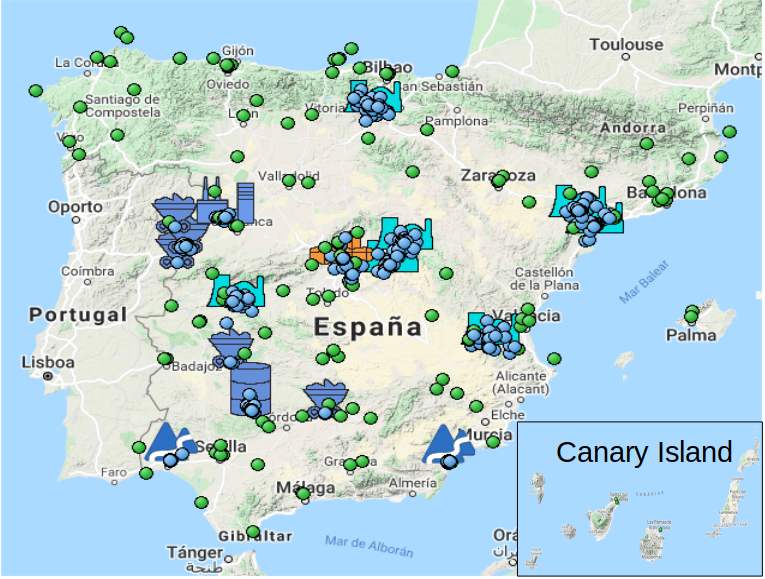
\includegraphics[width=\textwidth]{2Introduction/REM.png}  
    \caption{\label{subfig:REM}}
    \end{subfigure}
 \caption{Networks of automatic and sampling stations managed by the spanish CSN. (Above) Measurement locations of the REA \cite{REA}. The white box is the daily average of the gamma dose and the green box is the monthly average of the gamma dose. (Below) Measurement locations of the REM \cite{REM}. Blue dots are locations near nuclear facilities, and green dots are locations uniformly distributed throughout the country.}
 \label{fig:NetworksCSN}
\end{figure}

There are other networks that measure different parameters such as the concentration of $\ce{^{222}Ra}$ in the air. The measurements of all the networks complies with to the EUROTAM treaty \cite{100BqL}.
\end{enumerate}

The goal of this thesis and the \textit{TRITIUM} project is to develop a monitor capable of automatically measuring low levels of tritium in water in quasi-real time\footnote{Quasi-real time is an approximation of real-time measurements. It means a relatively small time, like ten minutes.}. This monitor is intended to be finally included in the REA.

Tritium is one of the radioactive isotopes routinely measured in REM tests and it is detected through the low-energy electrons produced in tritium beta decay, mainly using the liquid scintillation counter technique (LSC). Due to the limitations of the current tritium detection techniques, which will be described in section \ref{sec:StateOfTheArt}, the TRITIUM project has been recently created, the objective of which is to build a tritium detector based on scintillating fibers in contact with the water sample. The photons produced in these scintillating fibers are read out using photosensors, either photomultiplier tubes (PMTs) or silicon photomultipliers (SiPMs). 

The \textit{TRITIUM} collaboration is a international group consisting of a consortium of 6 different european institutions of 3 different countries: Portugal, France and Spain. The final emplacement of the \textit{TRITIUM} monitor is the Arrocampo dam (Extremadura, Spain), the water of which is used for the cooling system of the Almaraz nuclear power plant (NPP). This detector will be installed 4 km downstream from the Almaraz Nuclear Power Plant.

The monitor will be used to ensure that the tritium levels of the Arrocampo dam  water are below the legal limit of $100~\becquerel/\liter$ specified in the EURATOM Directive 2013/59/Euratom \cite{100BqL}. In addition, this will confirm the correct operation of the Almaraz NPP, since its malfunctioning may produce an increase of tritium activity released.

Tritium is one of the most abundantly produced radioisotope in a NPP, as it was verified in the United States Department of Energy complex, (U.S. DOE) \cite{FiberDetector1a, FiberDetector1b} and in several research facilities in China \cite{CommonEmissionTritium}, and also places close to them (ground water, surface water and process waste water).

%Generally, a nuclear reactor is characterized by high stability and, therefore, by a constant emission of radioactive isotopes. 
Tritium is produced in the water used for nuclear reactor cooling system of some NPPs by neutron capture of deuterium, existing in the heavy water ($\ce{D_2 O}$), semi-heavy water ($\ce{H D O}$) or deuterium created by neutron capture in usual water ($\ce{H_2 O}$). All these processes have a large probability to happen due to the huge neutron flux of the order of $10^{14} ~\ce{n} \, \cm^{-2} \second^{-1}$ in the nuclear reactor \cite{CrossSeccionNeutrons}. This tritium is finally released partially or totally to the environment in a quantity that depends on the reactor type as it is shown in Table \ref{tab:TritiumEmisionsNPPs}. The most common form in which tritium is released to the environment is $\ce{HTO}$ \cite{CommonEmissionTritium}.

\begin{table}[htbp]
\centering{}%
\begin{tabular}{lcc}
\toprule 
Reactor type & Gaseous discharge ($\giga\becquerel/$y) & Liquid discharge ($\giga\becquerel/$y)\tabularnewline
\midrule
\midrule 
PWR & $3.70\cdot 10^{3}$ & $2.59\cdot 10^{4}$ \tabularnewline
BWR & $1.85\cdot 10^{3}$ & $3.70\cdot 10^{3}$ \tabularnewline
HWR & $7.40\cdot 10^{5}$ & $1.85\cdot 10^{5}$ \tabularnewline
GCR & $7.40\cdot 10^{3}$ & $1.11\cdot 10^{4}$ \tabularnewline
\bottomrule
\end{tabular}
\caption{Emission of tritium per year from different types of nuclear reactors: Pressurized Water Reactor (PWR), Boiled Water Reactor (BWR), Heavy Water Reactor (HWR) and Gas-Cooled Reactor (GCR) \cite{CommonEmissionTritium}.}
\label{tab:TritiumEmisionsNPPs}
\end{table}

NPPs are operational since more than 60 years and, nowadays, they are essential for providing a large part of the electric power used all over the world (more than 20\% in Spain \cite{PercentageEnergySpain} and more than a 10\% in the world \cite{PercentageEnergyWorld}). Although the Spanish government is planning to progressively shut down all NPP, there are other countries like China \cite{60ReactorsChina} or United States (USA) \cite{35MillionsUSA} that promote their use. NPPs are a profitable investment since they are one of the cheapest source of energy production. Their energy production rate is stable as this doesn't depend on meteorological parameters. Moreover, NPPs do not emit greenhouse gases. Although there are alternative energy sources which are being developed quickly (photovoltaic, wind, tidal energy, etc.), as well as other concepts of energy production and saving (local production, solar roofs, energy efficiency, smart cities, etc.), they are currently not developed enough to fully cover the population needs. On the other hand, NPPs still have some important issues such as the contamination of fresh water from uranium mining, the nuclear waste produced, the nuclear proliferation or the risk of radioactive contamination from accidents as happened in the past: Chernobyl, Fukushima and Three Mile Island \cite{ThreeMileIsland}.

In any case, world nuclear energy production is most likely not going to be stopped in the next decade. In fact, the United States Energy Information Administration (U.S. EIA) expects a future increase of nuclear energy production \cite{EIAOutlook}. Therefore the development of  different types of alarm systems is an important investment. Safety is not a negotiable aspect and there must be safeguards that warn us of any malfunction of a nuclear power plant. Our objective is to ensure that the levels of tritium in the analyzed water are below the Spanish legal limit. It means that this monitor could be used in many different places with radioactive facilities like the future fusion power plants\footnote{The International Thermonuclear Experimental Reactor, ITER, will need up to several tens of kilograms of tritium to function, which correspond to various $\tera\becquerel$ of tritium.}, nuclear research facilities\footnote{Tritium is one of the main emissions from these sites \cite{FERMILAB}, \cite{BrookHavenNationalLaboratory}.} or tracking the pathway of tritium discharges to ground water \cite{TrackingTritium}. 

%which is normally done by liquid scintillation counter technic (LSC). This technic has a very good detection capability and precision but it has the inconvenient of providing a delayed results of about 1-2 days or even more. Liquid scintillation technique for the tritium measurement will be presented in section \ref{sec:StateOfTheArt}.